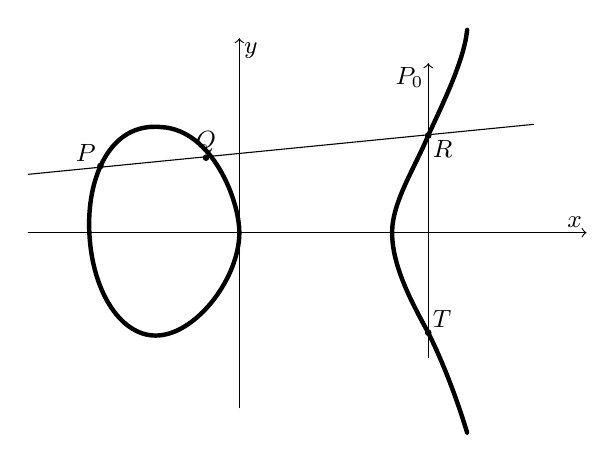
\begin{tikzpicture}[x=1bp,y=-1bp,line cap=round,line join=round,
  every node/.style={inner sep=1.5pt,font=\small}]
  \draw[->] (0,73) -- (201,73) node[above left] {$x$};
  \draw[->] (76,136) -- (76,3) node[below right] {$y$};
  \draw[->] (144,118) -- (144,12) node[below left] {$P_0$};
  \draw (0,52) -- (182,34);
  \draw[line width=1.6pt] (76,73)
    .. controls (76,61) and (66,36) .. (48,35)
    .. controls (29,33) and (21,54) .. (22,73)
    .. controls (23,95) and (34,111) .. (47,110)
    .. controls (61,109) and (76,89) .. cycle;
  \draw[line width=1.6pt] (158,0)
    .. controls (157,11) and (149,27) .. (144,38)
    .. controls (139,50) and (131,62) .. (131,73)
    .. controls (131,85) and (138,98) .. (144,109)
    .. controls (150,121) and (155,135) .. (158,145);
  \foreach \x/\y/\spot/\where in {26/49/P/above left,64/46/Q/above,
      144/38/R/below right,144/109/T/above right}
    \fill (\x,\y) circle[radius=1.2bp] node[\where] {$\spot$};
\end{tikzpicture}
